\documentclass[11pt,dvipdfmx]{jarticle}

\usepackage{eee}
\usepackage{subfig}

\renewcommand{\labelenumi}{\alph{enumi}}
\renewcommand{\labelenumii}{\roman{enumii}}

\begin{document}
% トップページを書く
\begin{jikkenTitle}
	\gakunen{3} % 学年を記述。この行で全体の枠を表示
	\numTitle{1}{電気電子計測} % 実験番号、タイトルを記述
	\subTitle{} % サブタイトルがあれば記述
	\jikkenbi{令和 4年5月12日(木)} % 実験日を記述
	\jikkenbiII{平成  年  月  日(  )} % 実験日を記述(二日目がある場合。ない場合はこの行をコメントアウト)
	\kyoudou{共同実験者名} % 共同実験者名を記述
	\kyoudouII{} % その他の共同実験者名を記述
	\yoteibi{5/19}% 予定日を記述
	\yoteibiII{}% 予定日2を記述
	\yoteibiIII{}% 予定日3を記述
	\hanNumberName{1}{3317}{杉山 滉太} % 班番号・学生番号・氏名を記述。この行でタイトルページの描画を終了
\end{jikkenTitle}

\section{目的}
本実験では
\begin{itemize}
	\item LabVIEWとMyRIOを使用して、素子の電圧電流特性について自動計測の方法を習得する。
	\item 測定データから近似直線式の傾き、切片を求める計算方法を習得する。
	\item 電圧電流特性から抵抗値を求める方法について習得する。
\end{itemize}
ことを目的とする。

\section{原理}
\subsection{LabVIEW}
LabVIEWは、各種計測器やmyRIOなどを用いて自動計測や制御を実装するためのグラフィカルユーザーインターフェイスのプログラミング言語である。
主な特徴は、ビルトインされた仮想計測器(以下VI)で、オシロスコープやマルチメーターなどの計測器と似た外観や機能をコンピューター上へ作成するというものである。
VIは、フロントパネル、ブロックダイアグラム、アイコン-コネクタという3つ主要素から構成される。
プログラミングは、ブロックダイアグラム上にアイコンを配置し、各アイコン間のコネクタをつなぐ形で行う。

\subsection{myRIO}
myRIOは、デュアルコアのARM Cortex-A9 リアルプロセッサとカスタマイズ可能なXilinx FPGA・アナログプロセッサの駆動するプログラミング言語には、LabVIEWを用いる。
LabVIEWとmyRIOを用いることにより、制御、ロボット、メカトロニクス、組込などを容易に実現することができる。

\subsection{myRIO ブレッドボードアクセサリ}
myRIOの拡張ポートに接続可能なブレッドボードアクセサリである。
myRIOの5V、3.3V、GND端子及びAnalog I/O、Digital I/Oの端子が、ブレッドボード上に結線した回路とヘッダにマッピングされている。
そのため、ブレッドボード上に結線した回路とヘッダとをジャンパ戦で結線することにより、回路への入出力制御および計測がmyRIOを用いて容易に実行することができる。

\subsection{真値と誤差及び相対誤差(誤差率)}
\subsubsection{真値}
真値とは、測定量(測定値ではない)が単位の何倍であるのかを示している値である。
真値は必ず存在すると仮定しても我々は真値そのものは知ることができず、ただその存在する範囲を推定することが出来るだけである。

\subsubsection{誤差及び相対誤差}
誤差は\weq{gosa}で定義される。
\begin{eqnarray}
	誤差 = 測定値 − 真値 
	\label{eq:gosa}
\end{eqnarray}
また、相対誤差とは真値に対する誤差の比である。
但し真値は分からないので、通常は\weq{soutaigosa}のように誤差が小さいとして真値の代わりに測定値で割る。
\begin{eqnarray}
	相対誤差 = \frac{誤差}{真値} \simeq \frac{誤差}{測定値}
	\label{eq:soutaigosa}
\end{eqnarray}

\subsection{統計処理(正規分布・平均値・標準偏差)}
\subsubsection{正規分布}
左右対称の釣鐘型に値が分布しているのを正規分布といい、山の頂点に平均値がくる。

\subsubsection{平均値}
平均値とは$N$個全てのデータの総和を$N$個で割って得られる値で、\weq{heikinchi}で表すことができる。
\begin{equation}
	\bar{y} = \frac{1}{N}\sum^N_{i = 1}y_i
	\label{eq:heikinchi}
\end{equation}		

\subsubsection{標準偏差}
標準偏差とは平均値を基準に各測定量がどれほどのばらついているかを定量的に表す値で、\weq{hyoujunhensa}で表すことができる。
\begin{equation}
	\sigma = \sqrt{\frac{1}{N - 1}\sum^N_{i = 1}(y_i - \bar{y})^2}
	\label{eq:hyoujunhensa}
\end{equation}	

\subsection{近似直線(最小二乗法)}
%。
2つの測定データ$y, x$間に一次方程式の関係があるとし、
\begin{equation}
	y = ax + b
	\label{eq:aiu}
\end{equation}
の傾き$a$、切片$b$を測定データから尤もらしい値にすることを考える。
その際に、
\begin{eqnarray}
	E &=& \sum\limits_{i=1}^{N} \varepsilon^2_i \nonumber\\
	&=& \sum\limits_{i=1}^{N} \bigl( y_i - f(x_i)\bigr)^2\nonumber\\\
	&=& \sum\limits_{i=1}^{N} \bigl( y_i - (ax_i+b)\bigr)^2
	\label{eq:error}
\end{eqnarray}
を最小にする$a$、$b$を求める。
これを最小二乗法といい、誤差を伴う測定値の処理においてその誤差の二乗の和を最小にすることで、最も確からしい関係式を求める方法である。
\begin{eqnarray}
	\frac{\partial}{\partial a}E(a,b) &=& 0\\
	\frac{\partial}{\partial b}E(a,b) &=& 0
\end{eqnarray}
から得られる方程式を、それぞれ$a$、$b$について解けば良く、それぞれの解を得るための方程式は次の2つを用いることになる。
\begin{equation}
	a = \frac{\sum_{n=1}^{n}(x_i -\bar{x})(y_i-\bar{y})}{\sum_{n=1}^{n}(x_i-\bar{x})^2}
	\label{eq:saisyou1}
\end{equation}
\begin{equation}
	b = \bar{y}-\frac{\sum_{n=1}^{n}(x_i -\bar{x})(y_i-\bar{y})}{\sum_{n=1}^{n}(x_i-\bar{x})^2} \bar{x}
	\label{eq:saisyou2}
\end{equation}

\section{方法}
\subsection{使用器具}
今回の実験で使用した器具を表\ref{tab:tools}に示す。
\begin{table}[hbtp]
	\caption{使用した実験器具}
	\label{tab:tools}
	\centering
	\begin{tabular}{|c|c|c|}
		\hline
		製品名 & 製造元 & 型番\\
		\hline \hline
		ノートパソコン & iiyama & NKNK50SZ0000K0099\\
		\hline
		MyRIO & ANATEL & 30877F9\\
		\hline
		MXP Breadboard & DIGILENT & D537697\\
		\hline
		LabVIEW2019 & NATIONAL INSTRUMENTS & ver:19.0.1f3\\
		\hline
	\end{tabular}
	
\end{table}

\subsection{実験手順}
	\subsubsection{課題実験1}
		\begin{enumerate}
			\item ブレッドボートを図\ref{fig:circuit1}のように組み立てMyRIOのAポートに接続する。
			\item 図\ref{fig:program1}のようなプログラムを書き図\ref{fig:circuit1}の端子を、GND,3.3V,5Vになぎ変えながら3回実行する。
			\item 出力した結果をもとにエクセルを使用し、平均値と標準偏差を求めた。
		\end{enumerate}

	\subsubsection{課題実験2}
		\begin{enumerate}
			\item ブレッドボートを図\ref{fig:circuit2}のように組み立てMyRIOのAポートに接続する。
			\item 図\ref{fig:program2}のようなプログラムを書き0Vから5Vまで0.5V刻みでAO0から出力する。
			\item AO0の値、AI0の値、AO0からAI0を引いた値、通し番号を出力しExcelにまとめる。
			\item まとめたExcelから二乗平均平方誤差を求める。
		\end{enumerate}



			\begin{figure}[hbtp]
				\begin{tabular}{cc}
					\begin{minipage}[c]{0.5\linewidth}
						\centering
						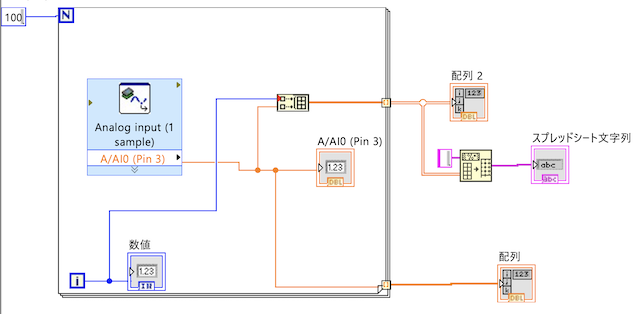
\includegraphics[keepaspectratio,scale=0.45]{circuit1.png}
						\caption{課題実験1のプログラム}
						\label{fig:program1}
		
					\end{minipage}&
		
					\begin{minipage}[c]{0.5\linewidth}
						\centering
						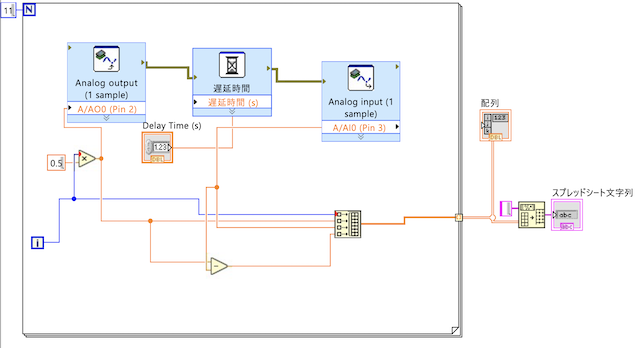
\includegraphics[keepaspectratio,scale=0.4]{circuit2.png}
						\caption{課題実験2のプログラム}
						\label{fig:program2}
						
					\end{minipage}\\


					\begin{minipage}[c]{0.5\linewidth}
						\centering
						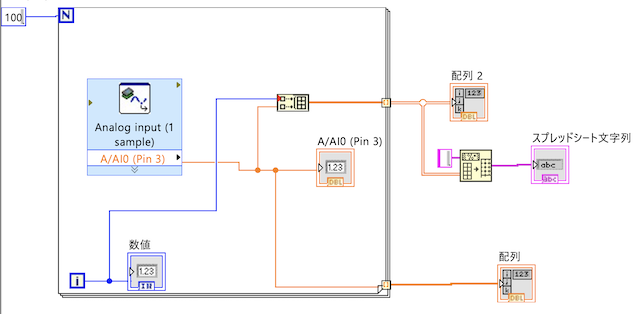
\includegraphics[keepaspectratio,scale=1.2]{circuit1.pdf}
						\caption{課題実験1の回路図}
						\label{fig:circuit1}
						
					\end{minipage}&
		
					\begin{minipage}[c]{0.5\linewidth}
						\centering
						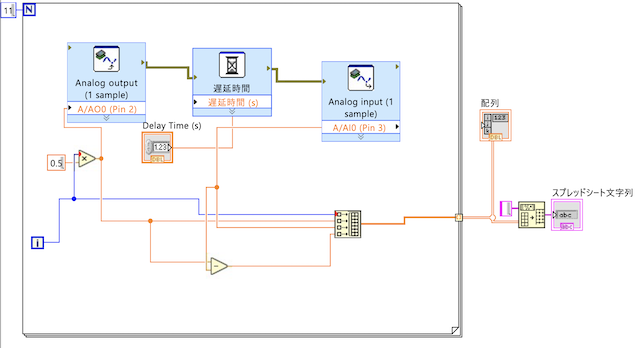
\includegraphics[keepaspectratio,scale=1.2]{circuit2.pdf}
						\caption{課題実験2の回路図}
						\label{fig:circuit2}
						
					\end{minipage}


				\end{tabular}
			\end{figure}


\section{結果}
			
\section{考察}
\section{結論}

\begin{thebibliography}{9}%参考文献数が10以上の場合は9を99に変更
	%\bibitem{xxx}の引用を本文中で行うには\cite{xxx}と記述。
	\bibitem{a} 著者名, 書名,出版社,発行年.
\end{thebibliography}


\end{document}